\documentclass{article}

\usepackage[left=2.54cm,bottom=2.54cm,top=2.54cm,right=2.54cm,nohead,nofoot]{geometry}
\usepackage{listings}
\usepackage{graphicx,epsfig,latexsym,subfig}
\usepackage{amsmath,amsthm,amsfonts,amscd,amssymb,bm,mathtools,setspace,fancyhdr,commath,mathrsfs,mathtools,dsfont,tikz-cd,soul,booktabs,longtable,diagbox}
\usepackage{tikz}
\usepackage{multicol}
\usepackage{tkz-euclide}
\usetkzobj{all}
\usetikzlibrary{calc,decorations.markings}
\everymath{\displaystyle}
\usepackage[toc,page]{appendix}
\usepackage{spverbatim}
\usepackage{float}

\pagestyle{empty}
\renewcommand{\headrulewidth}{2pt}
\cfoot{\thepage}
\cfoot{\vspace{0.4cm} \thepage}

\title{Santander Product Recommendation}

\begin{document}
	\maketitle
	\begin{center}\begin{Large} Xinyi Hou,
			Yingxi Yu,
			Yuan Xu,
			Wenyu Li,
			Qiaojuan Niu,
			Huiyu Bi,
			Meng Li,
			Zhongyu Fan,
			Aoran Zhang,
			Yuan Tian,
			Miao Wang,
			Markham Anderson,
			Bowen He,
			Charlton Lin,
			Zoran Dabic \end{Large}\end{center}
	\begin{spacing}{1}
		\begin{large}

\begin{abstract}
	 Our topic is specified in the Santander Kaggle competition. Our goal is to predict which products customers will purchase next month based on behavioral and demographic data from the 1.5 years. To solve this, we use four different machine learning methods: logistic regression, SVM, random forest and XGBoost. Since the data size is large and there is no clear response variable in the training set, different subteams use different subsets of the original training set and build their own response variables. Thus, it is difficult to compare the four different methods. We find that all four methods could provide reasonable predictions and this would help the Santander Bank to build a more effective recommendation system.
\end{abstract}

\section{Author Contributions}


\begin{multicols}{2}

\textbf{XGBoost} \\
Xinyi Hou: Lead the project as a whole, pre-processed data, tune parameter and wrote final abstract. \\
Yingxi Yu:  Wrote the model code,tune parameter and made the powerpoint. \\
Wenyu Li: Wrote model code, tune parameter and the group's report. \\
Yuan Xu:  Worked on the group's report and tune parameter. \\
\textbf{Random Forest} \\
Charlton Lin: Created the flattening and feature engineering, and worked on conforming to Kaggle standards. \\
Qiaojuan Niu : Created the Random Forest model and code to clean the data. \\
Zoran Dabic: Subgroup report, compiled full report, feature engineering, ran the model and generated results. \\
\textbf{SVM} \\
Data processing:Aoran Zhang, Huiyu Bi \\
Data analysis and interpretation: Meng Li, Zhongyu Fan, Huiyu Bi \\
Model analysis and interpretation:Aoran Zhang, Meng Li \\
Drafting the article: Aoran Zhang, Meng Li, Huiyu Bi, Zhongyu Fan \\
Critical revision of the article:Aoran Zhang, Zhongyu Fan \\
\textbf{Logistic Regression} \\
Bowen He:  Data analysis and interpretation, code to create purchase history variables, feature engineering\\
Yuan Tian:  Data analysis and interpretation, data cleaning code, generated the idea of ETL process, i.e. defining labels and feature space, and revised the report. \\
Miao Wang:  Data analysis and interpretation, code to create response variables, feature engineering, and revised the report. \\
Markham Anderson: Wrote the subgroup report, data processing, created Logistic regression model, wrote classifier code and evaluated its performance. \\

\end{multicols}

\newpage

\section{Introduction}
The logistic regression and SVM subteams both build 24 classifiers for 24 products and the accuracy is high, which is above 0.9. However, we cannot say these two classifiers are powerful, because the training set is quite unbalanced. The random forest and XGboost both build only one multi-classifier model. The accuracy for these two are 0.90 and 0.63. As these two subteams use different data cleaning method and response variable, we cannot say random forest is better than XGboost.


This paper introduces four machine learning methods. In each sub parts, we will introduce the way we clean the data, models and results, and the discussions of this method.

\section{XGBoost}


\subsection{Data Pre-processing}

\noindent \indent Since there are many missing values and outliers, the first thing is to delete 27334 records with 9 consecutive NA values and extreme values (for an instance, the 99 percent quantile of the age variable is 88 years old). Then, we decide to only use 32 features to predict the response. For the \verb|"age"|, \verb|"antiguedad"| and \verb|"renta"|, we cut them into 5 intervals and they also become categorical features now.

The response is the additional product which the customer would add in the next month. If the customer adds more than one product, we only randomly pick one of them. To make the data size smaller and the problem easier, we subset the samples with nonzero response, which means we only consider the records with additional product.

\subsection{XGBoost Algorithm}

\noindent \indent To find the best parameters given the training data, we need to define a so-called objective function. Here for XGBoost algorithm, the objective function contains two parts: training loss and regularization.
\[
Obj(\Theta) = L(\theta) + \Omega(\theta)
\]
where $L$ is the training loss function, and $\Omega$ is the regularization term. The training loss measures how predictive our model is on training data. The regularization term controls the complexity of the model, which helps avoiding overfitting. We define these two items as:
\[
L(\theta) = \sum_{i}(y_i - \hat{y_i})^2 \ \ \ \ \ \
\Omega(f) = \gamma T + \frac{1}{2}\lambda\sum_{j = 1}^{T}(w_j)^2
\]




\subsection{Results}

\noindent \indent Contrary to other groups, we only apply the algorithm once and fit a multi-classifier model. We randomly pick 70\% of the data for training, and the rest for testing. By changing the main parameters \cite{xg3} max.depth among 5, 6, 7, the number of trees among 10, 50, 100, and the step size among 0.1, 0.5, 1, we get the results displayed in the tables as below.
\begin{table}[h]
\centering
\caption{Accuracy for Training Data}
\label{Accuracy for Training Data}
\begin{tabular}{cccccccccc}
\hline
max.depth       & \multicolumn{3}{c}{5} & \multicolumn{3}{c}{6} & \multicolumn{3}{c}{7} \\ \hline
\# of trees     & 10    & 50    & 100   & 10  & 50       & 100  & 10    & 50    & 100   \\
step size = 0.1 & 62.06\%    & 62.45\%     & 62.79\%     & 62.32\%    & 62.77\%         & 63.10\%      & 62.54\%     & 62.89\%      & 63.24\%      \\
step size = 0.5 & 62.47\%    & 63.37\%       & 63.46\%      & 62.79\%   & 63.70\%  & 64.48\%     & 62.97\%       & 64.20\%      & 64.32\%      \\
step size = 1   &38.30\%       & 31.70\%      &35.07\%       &18.31\%     & 36.78\%         &36.65\%      &30.46\%       &46.37\%       &44.31\%       \\ \hline
\end{tabular}
\end{table}

\begin{table}[h]
\centering
\caption{Accuracy for Test Data}
\label{Accuracy for Test Data}
\begin{tabular}{cccccccccc}
\hline
max.depth       & \multicolumn{3}{c}{5} & \multicolumn{3}{c}{6} & \multicolumn{3}{c}{7} \\ \hline
\# of trees     & 10    & 50    & 100   & 10  & 50       & 100  & 10    & 50    & 100   \\
step size = 0.1 & 62.09\%      & 62.37\%     & 62.63\%      &62.30\%     & 62.59\%       & 62.80\%      & 62.45\%      & 62.76\%      & 63.10\%      \\
step size = 0.5 & 62.41\%     & 62.80\%     & 62.92\%      & 62.57\%    &62.85\%     & 62.94\%   & 62.61\%      & 62.88\%      & 62.89\%      \\
step size = 1   &38.45\%       & 31.80\%      & 35.29\%      &18.30\%     & 36.72\%         &  36.98\% &30.61\%       &46.55\%      &44.45\%     \\ \hline
\end{tabular}
\end{table}

\noindent \indent From the above tables, we can see the highest accuracy for the training set is 64.48\%, and for the test set is 62.94\%, when max.depth = 6, the number of rounds(the number of trees) = 100 and the step size = 0.5.  When step size = 1, the accuracy for training and test set are about 40\%, which means this situation is not ideal.

\noindent \indent According to the best parameters that lead to highest test accuracy, we got the feature importance plot  as below. The feature importance figure shows the different gains for different features. From the plot, we can see features \verb|"ind_cno_fin_ult1"|, \verb|"ind_recibo_ult1"| and \verb|"ind_cco_fin_ult1"| obtain the first three highest gains.

\begin{figure}[H]
\centering
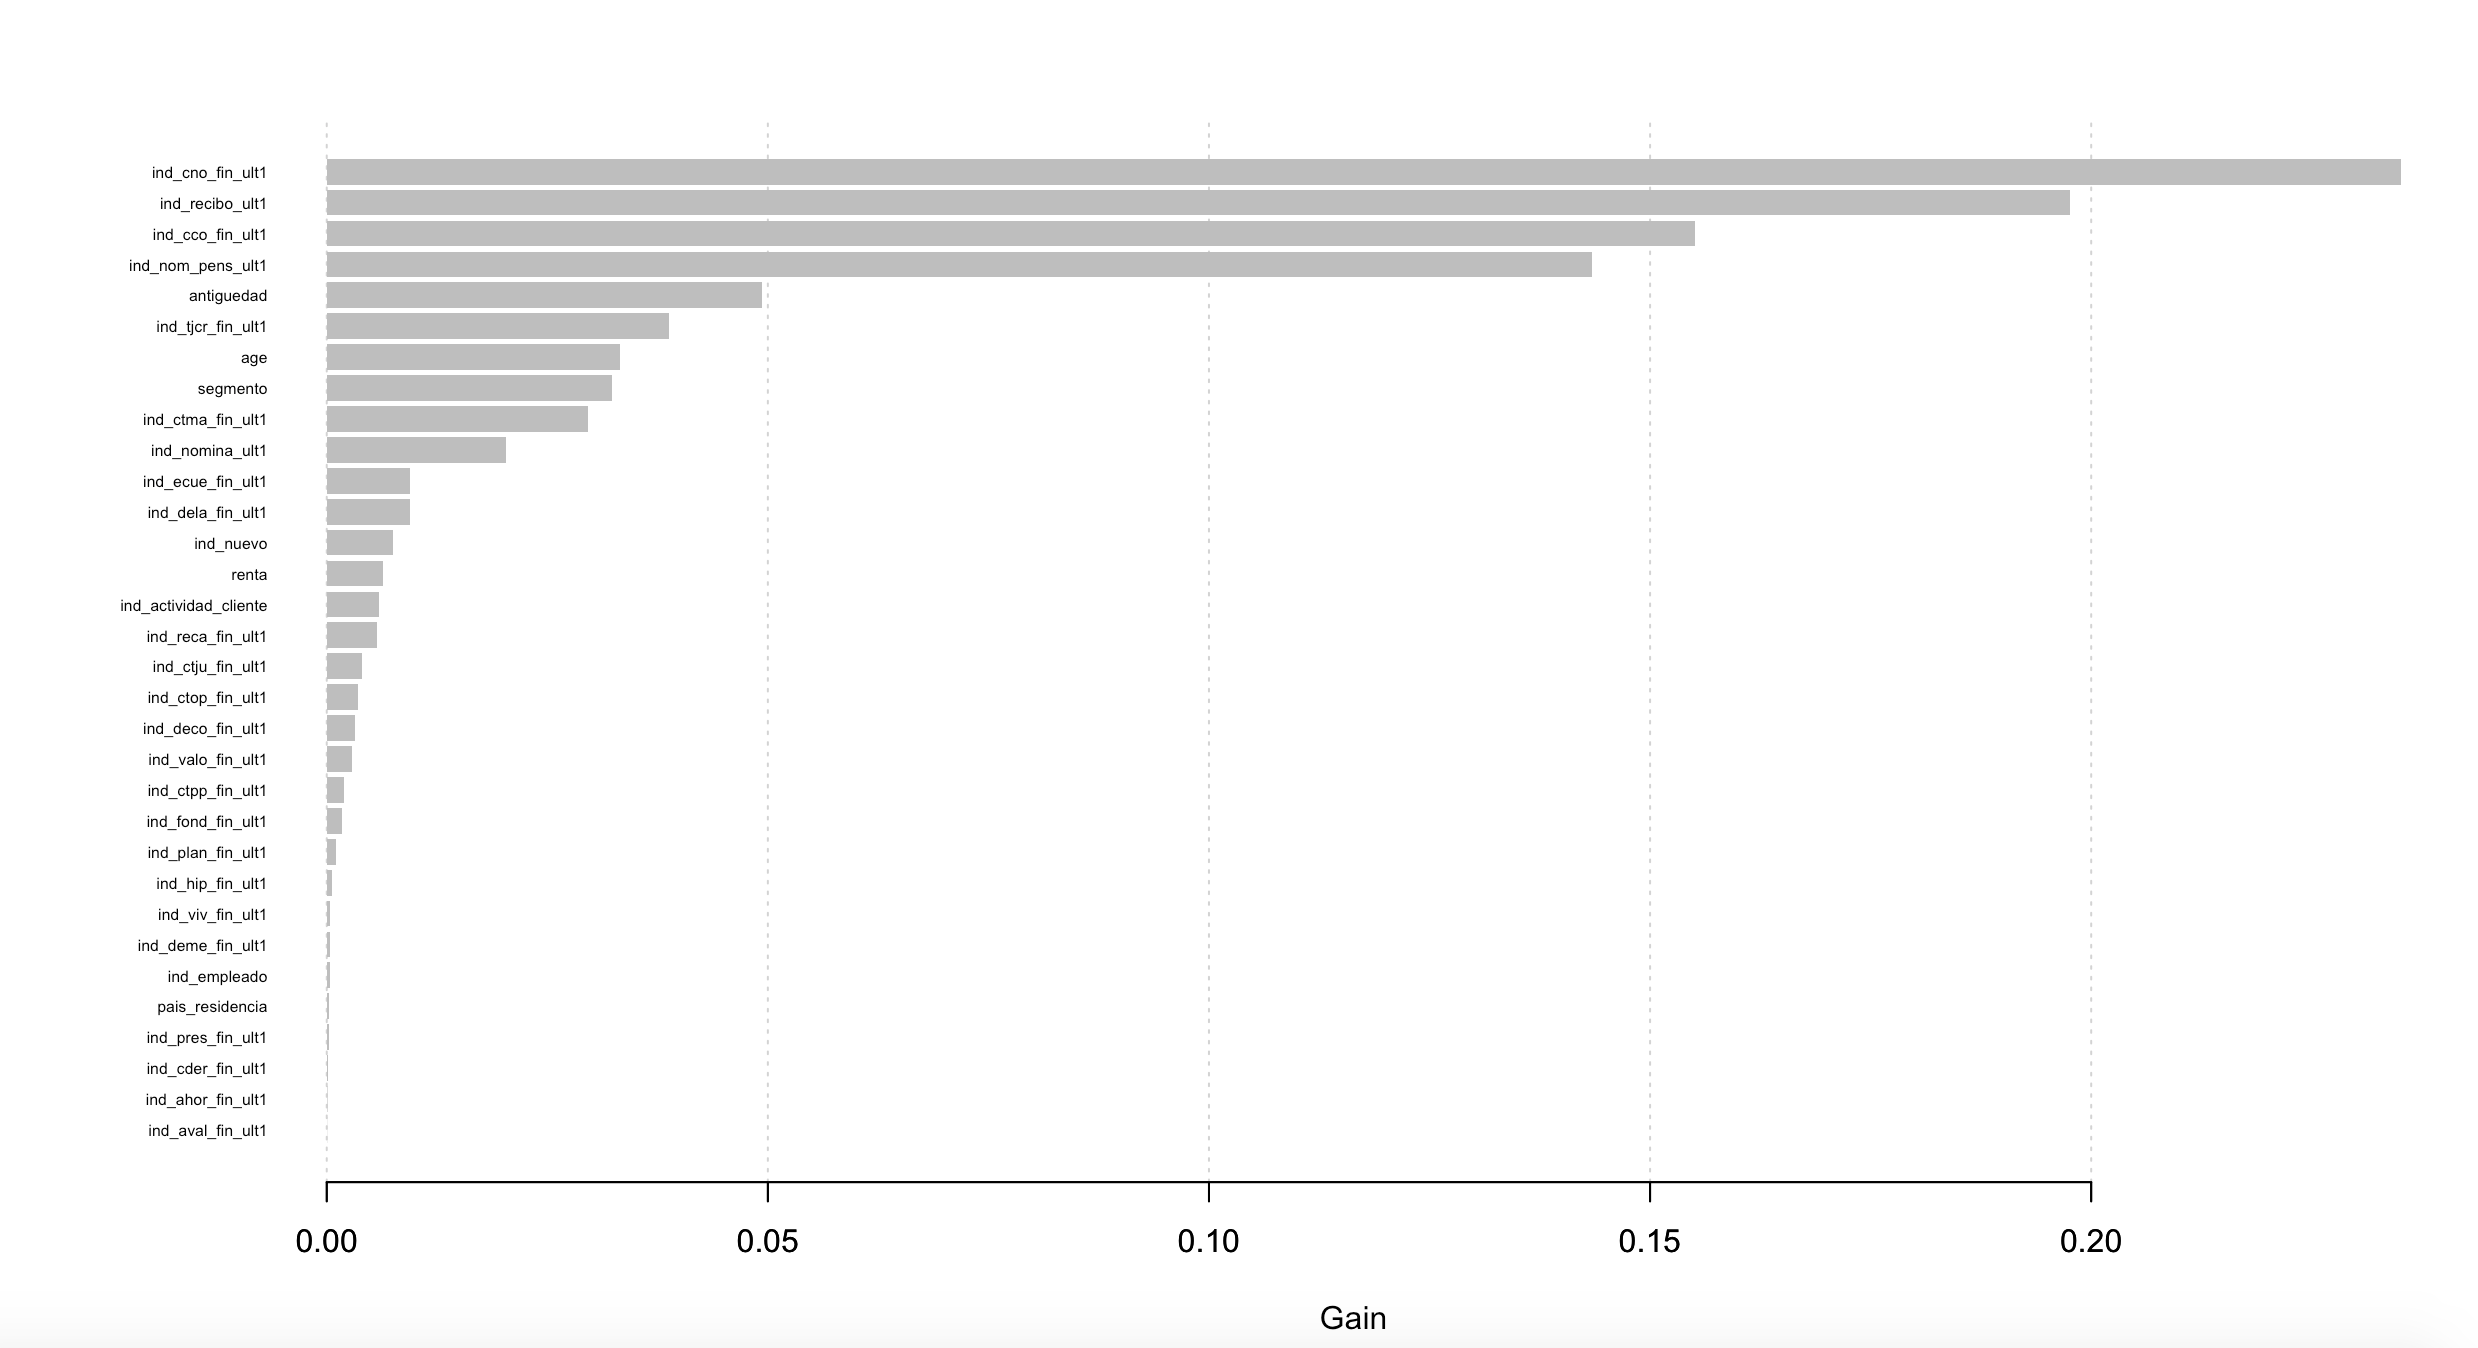
\includegraphics[width = 100mm]{113.png}
\caption{Feature Importance}
\end{figure}

\subsection{Discussion}

To make the model better, we could dive deeper. For example, we may consider more features and not cut some variables into intervals. We may also take the history length of the used products into account.

Due to the vague description of the problem, we are not sure how many new products to predict for each user. In fact, most members seldom tried new products based on historical records. Some valuable information might be lost since we drop some predictors and only pick one new product every time (if more than one).

\section{Random Forest}
	
\subsection{Data Analysis}

Random forests do not handle time series very well. Had we not transformed the data we would have had to worry about how the training and testing subsets were selected to ensure that future data is not used to predict past data. In addition, a decision tree cannot split on a non repeating independent variable such as time to produce any useful results. So we would have had to generate features to capture the time trend.

In general we filled NA values with the mode of the value across all customers if it was categorical. We moved the outliers for age to the median of the age category (above or below 30).
For testing, we flattened the time-series data such that each customer only had 1 row. We generally used aggregates of the users' columns, such as the mode for that user over time.
Since Kaggle does not provide true classes in 2016-6, our testing set uses product classes from 2016-5 as true predictor variables for each customer.

\subsection{Method}

\paragraph{Random Forest}
We use a random forest model with 100 trees. A RF model uses decision trees as weak predictors of the response variable to produce a strong predictor in the random forest. Each tree is produced on a random subset of samples with replacement and would otherwise suffer from over fitting and high variance. At each split a random subset of features without replacement is used to find the best split. Each tree produces a classification and the mode of the classifications becomes the forest's overall classification for the sample. However for our model, sklearn instead averages the probability of predicting a class across all trees.\cite{rnSKlearn}  The out of bag samples for each tree is used to test the tree and provide an unbiased estimator of the classification error.\cite{rnLeo}

\paragraph{Choosing the Random Forest}

Random forests scale very well with large input sizes. The bagging process results in a strong predictor over all the trees. The random forest can also handle our categorical variables directly so we will not have to generate dummy variables for the categories. Additionally, the random forest supports multi-label classification so we don't have to separately fit model for each response variable.

\subsection{Results}

\begin{multicols}{2}
\begin{table}[H]
	\centering
	\begin{tabular}{|c|c|c|c|}
		\hline
		\backslashbox{Trees}{Depth} & 10 & 100 & $\infty$ \\
		\hline
		1 & 0.7434 & 0.8594  & 0.8594 \\
		10 & 0.8465 & 0.8956  & 0.8956 \\
		100 & 0.8518 & 0.9044  & 0.8921 \\
		\hline
	\end{tabular}
	\caption{Model Accuracy vs \# of Trees and Tree Depth}
	\label{tab:my_label}
\end{table}

\begin{figure}[H]
	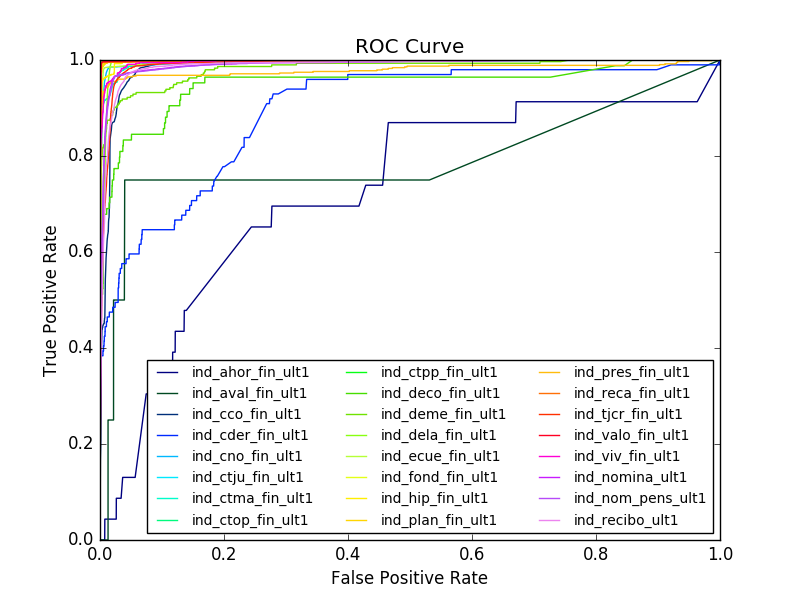
\includegraphics[width = 7cm]{ROC.png}
	\caption{ROC for 100 trees with depth of 10}
\end{figure}


\end{multicols}

\subsection{Discussion}

As expected our classification accuracy grows with tree size and depth. However due to the flattening process we may have lost information about time trends relating to customer behavior. To improve the model we could have used a categorical variable for the month to capture seasonal effects.

\subsection{Reproduction}
Run \texttt{fixdata.py} to generate cleaned data, and then run \texttt{flatten.py} to flatten data. Run \texttt{fitmodel.py}. To adjust parameters, modify \texttt{fitmodel.py}. For the final model run \texttt{kaggletest.py} which generates a model using all the data.

\section{SVM}

\subsection{Data Processing}
\textbf{Independent Variable Selection:} To increase model efficiency and accuracy we removed irrelevant features. (1) We delete discrete variables with too many classes since they are hard to transform into dummy variables. (2) We leave out independent variables with repeated information. (3) We removed variables with predominantly missing values.\cyte{paper1}

According to these three  rules, we remove : pais\_residencia, fecha\_alta, indext, conyuemp, canal\_entrada, tipodom, cod\_prov and nomprov.

\textbf{Missing values}: For the cases having missing values in any of the 24 dependent variables, we remove them. This case occurs $<$ 1\% of the time and has no obvious pattern.

\textbf{Data Transformation}: We transform categorical variables to dummy variables, and standardize the continuous variables.

\subsection{SVM Model}

SVM is the supervised learning model for classification. With associated learning algorithms, a line or a hyper-plane is found to classify the data. \cite{book}

We want a classifier that is less sensitive to outliers. To do so, we introduce “slack variables” that allow samples to be misclassified. We also utilize kernels.

Decision function:
$$f(x) = \displaystyle\sum_{i}\alpha_i\Phi(x_i)\Phi(x)+b = \displaystyle\sum_{i}\alpha_{i} K(x_i, x)+b$$, where $K(x_i, x)$ is the Kernel function.

Dual formulation:
$$min P(w,b) = \frac{1}{2}(||\displaystyle\sum_{i=1}^{m}\alpha_i\Phi(x_i)||)^2 + C\displaystyle\sum_{i}H_{i}[y_{i}f(x_i)]$$

\subsection{Results}

For each of the 24 estimations, the accuracy is higher than 99\% which indicates a high performance of the model.

\subsection{Discussion}

However, scrutiny of the data reveals simply focusing on the accuracy is not reasonable. For most dependent variables, the negative class 0 dominates. Thus, since the majority of predictions are 0, incorrect 1 predictions do not influence accuracy much. To examine this idea, we choose 3 dependent variables with asymmetric distribution in 0s and 1s, and then use ROC and PRC to exhibit the results:

\vspace{5mm}
\begin{tabular}{| l | l | l |}
	\hline
	& Really True & Really False \\ \hline
	Predicted True & 0 & 0 \\ \hline
	Predicted False & 558 & 99442\\
	\hline
\end{tabular}
\vspace{5mm}

Although accuracy is very high, the model is useless since we are interested in helping the bank recommend products. Thus, true positives are necessary. Failing to consider other metrics of evaluation like precision and recall would lead to an unjustified model. Here the recall is 0 and the precision is NA because there is not a single observation being classified as 1. The reason is that the negative class 0 is predominant in "ind\_cco\_fin\_ult1" and the model tends to classify everything as 0, so many true 1’s are incorrectly classified 0. The results are even worse for the other two variables as class 1's are sparser.

ROC and PRC curve for "ind\_cco\_fin\_ult1" , "ind\_fond\_fin\_ult1" and "ind\_deme\_fin\_ult1"

\begin{multicols}{2}
\vspace{5mm}
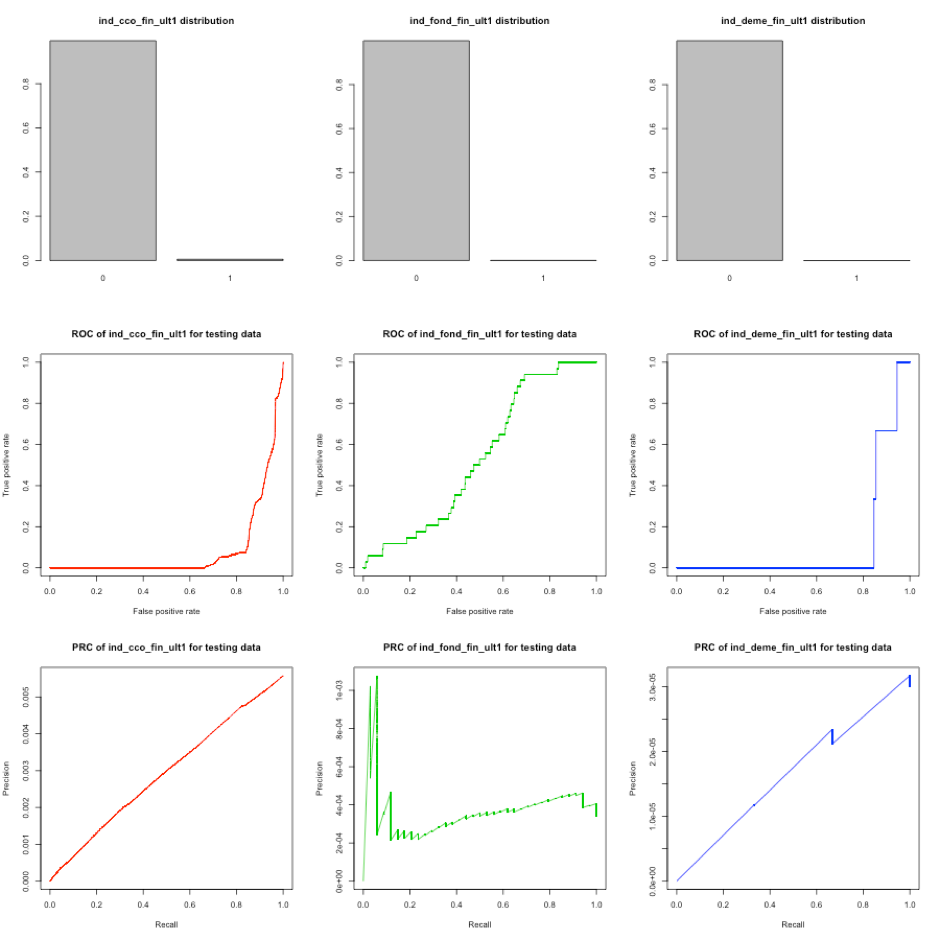
\includegraphics[scale = 0.3]{ROCandPR.png}
\vspace{5mm}

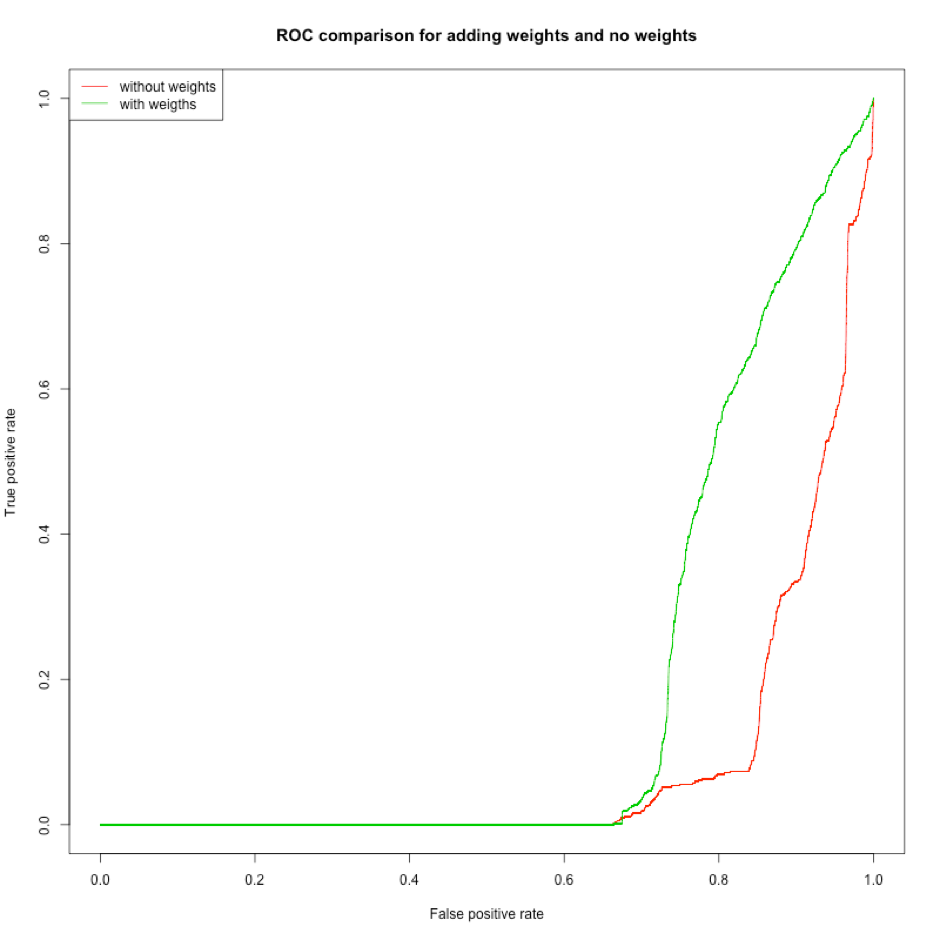
\includegraphics[scale = 0.3]{ROCwithandwithoutweights.png}


\end{multicols}

 To solve this problem, we add higher weights to the minority class which would encourage the model to be gear towards classifying 1 as 1 and add some penalty for model to predict 0. The results are as follows. It is shown that all class 1’s are correctly classified! Now the precision and recall are 1.64\% and 100\%. But there is some inevitable trade offs as in general one of these two metric gets better, the other will get worse. Additionally, since we add more penalty when the model predicts 0, there are plenty of class 0 being misclassified which leads to accuracy decreasing to 66.51 as well as decreasing in specifity. However, in our case, recall should be the first priority as we do not want to lose any potential customers, we should accept this trade off. It is also worth noting that another downside is that the process for training model is more time consuming than before.

\vspace{5mm}
\begin{tabular}{| l | l | l |}
	\hline
	& Really True & Really False \\ \hline
	Predicted True & 558 & 33488 \\ \hline
	Predicted False & 0 & 65954\\
	\hline
\end{tabular}
\vspace{5mm}

\section{Logistic Regression}

\subsection{Defining a sample (features-to-label pair)}

With some ambiguity in the Santander description, we defined a sample (features-to-label pair) as the values for any two consecutive months for a single customer. The "date" of a sample refers to the earlier of these two months.

\subsection{ETL}

Our labels (Y-values) are 24 binary fields corresponding to the Santander products which a customer may have purchased. We determined when each product was purchased and set the corresponding Y-value to 1 if the purchase took place in the month after the date of the sample, 0 otherwise.

For the feature space (X-values), we did the following feature engineering. (1) For each product, we added a column to hold the number of months since the customer’s first purchase of that product. So in total, 24 columns contained the the purchase history for each customer, up to the given month. (2) The variable "fecha\_alta" was the date in which the customer first acquired a contract with the bank. We replaced it with a variable "memberdays" which holds the difference between this date and the sample date, i.e. "fecha\_dato". (3) We replaced categorical features with sets of binary features: one binary column for each category for a given feature. (4) A certain 27334 rows each had exactly 9 missing values in all the same columns. We eliminated the troublesome rows. About 10\% of the samples were missing $renta$; so we filled the missing values by using averages based on province. \cite{paper2} (5) Some features were irrelevant for calculation, such as $tipodom$ (address type), and could be discarded easily. Others were used for organizing data but not for calculating regressions: $nomcodpers$ and $fecha\_dato$. $nom\_prov$ was redundant with $cod\_prov$, so we omitted the former.
 
\subsection{Limiting the Sample}

The data had grown to 39GB in memory. In order to turn out results quickly and avoid the cost of backtracking, we limited the size of the data with which we worked by taking a random sample from the output of our ETL. We experimented with samples of different size and eventually proceeded with a working set of 197968 ($1/2^6$ as many as we produced in ETL). We used a random 10\% of these samples as testing data.

\subsection{Regression}

We performed a logistic regression on each of the 24 products that a customer might have purchased. We used the sigmoid function $(1+e^{w^Tx})^{-1}$.

We performed logistic regression using an augmented error if $\lambda \times L_2norm$ (ridge regression). Naturally, we would use cross-validation to identify the best $\lambda$ for the data, but due to time constraints, we used our sense of the problem to decide on a $\lambda$ value of 0.1. If we were to redo this, we would perform 10-fold cross-validation over a range of possible $\lambda$'s and choose the one that produced the lowest validation error.

We considered a variable learning rate such as Newton's method or a rate that decayed as the iteration count grew. Ultimately, we used an implementation inspired by steepest descent: we began each weight-update with a learning rate of 0.1, which we supposed would be too large in many cases. \cite{book2} If the new weights produced an error larger than the previous one, we would try a learning rate half as large, and proceed from there in the fashion of a binary search for some time until we found a minimum error for the current gradient or until we reached some number of iterations.

\subsection{Results}

For the 24 products (i.e. regressions), we calculated the following mean-squared testing errors on our held-out data:

\begin{table}[h]\footnotesize
	\centering
	\caption{Held-out Data MSE}
	\label{my-label}
	\begin{tabular}{llllllll}
		\hline
		MSE = 0                            & ahor\_fin:  & cder\_fin: & deme\_fin: & hip\_fin:  & viv\_fin:  &                     &            \\
		& 0                    & 0          & 0          & 0          & 0          &                     &            \\ \hline
		0 \textless MSE \textless 0.001      & ctma\_fin:          & ctop\_fin: & deco\_fin: & fond\_fin: & plan\_fin: & reca\_fin:  & valo\_fin: \\
		& 0.000303            & 0.000455   & 0.000253   & 0.000253   & 0.000101   &  0.000707             & 0.000354   \\ \hline
		0.001 \textless MSE \textless 0.01 & cco\_fin:           & cno\_fin:  & ecue\_fin: & dela\_fin: & tjcr\_fin: & nomina:             & nom\_pens: \\
		& 0.006567            & 0.002576   & 0.001667   & 0.001061   & 0.005203   & 0.005607            & 0.006921   \\ \hline
		0.01 \textless MSE \textless 1     & ctju\_fin:          & ctpp\_fin: & recibo:    &            &            &                     &            \\
		& 0.999949            & 0.999899   & 0.011517   &            &            &                     &            \\ \hline
		MSE = 1                            & aval\_fin:          & pres\_fin: &            &            &            &                     &\\
		&                    & 1          &1           &            &            &                     & \\
		\hline
	\end{tabular}
\end{table}
The mean of these errors is 0.1685.

\subsection{Discussion}

\begin{multicols}{2}


The results of the logistic regressions are suspect. Testing errors range from 0 to 1, inclusive. Scarcity of data for certain products may explain the frequency of errors at these two extremes. In the original dataset, some purchases are so rare that it may be that our reduced dataset contains zero $1$'s for a given product, which would yield a testing error of zero.

Although limiting the dataset to $1/2^6$ of its original size may hurt generalization, we still have almost 200K samples to work with and only 419 features, well past the ten-times-the-VC-dimension rule of thumb.\cite{Amlbook}

In future, we might perform further feature reduction. On a typical example from our 24 regressions, 251 non-zero weights remained. Nevertheless, only 19 weights measured greater than 0.00001.

Our decisions for how to fill in missing values also likely contribute to some inaccuracy in our model.

\end{multicols}

\newpage

\begin{thebibliography}{9}

	\bibitem{xg1}
	Tianqi Chen, Carlos Guestrin
	\emph{XGBoost: A Scalable Tree Boosting System}. Preprint.

	\bibitem{xg2}
	\emph{Awesome XGBoost}.
	https://github.com/dmlc/xgboost/tree/master/demo

	\bibitem{xg3}
	\emph{XGBoost Parameters}.
	http://xgboost.readthedocs.io/en/latest//parameter.html

	\bibitem{rnLeo}
	Breiman, Leo and Cutler, Adele
	\textit{Random Forest}.
	\\\texttt{https://www.stat.berkeley.edu/~breiman/RandomForests/cc\_home.htm}

	\bibitem{rnSKlearn}
	Scikit Learn,
	\textit{Ensemble Methods}.
	\\\texttt{http://scikit-learn.org/stable/modules/ensemble.html}

	\bibitem{book1}
	Gareth James, Daniela Witten, Trevor Hastie, Robert Tibshirani, \textit{An Introduction to Statistical Learning}. New York, USA: Springer, 2013.

	\bibitem{book2}
	Trevor Hastie, Robert Tibshirani, Jerome Friedman, \textit{The Elements of Statistical Learning}. New York, USA: Springer, 2008.

	\bibitem{Amlbook}
	Yaser S. Abu-Mosta, Malik Magdon-Ismail, Hsuan-Tien Lin, \textit{Learning From Data: A Short Course}. New York, USA: AMLBook, 2012.

	\bibitem{book}Kevin, P. Murphy, \textit{Machine Learning: A Probabilistic Perspective}. London, England:The MIT Press, Cambridge Massachusetts, 2012.

	\bibitem{paper1}
	herkassky, Vladimir, and Yunqian Ma, \textit{Practical selection of SVM parameters and noise estimation for SVM regression}. Neural networks 17.1 (2004): 113-126.

	\bibitem{paper2}
	Yehuda Koren, Robert Bell, and  Chris Volinsky,
	\textit{Matrix Factorization Techniques for Recommender Systems}. IEEE Computer Society, 2009.
\end{thebibliography}

\end{large}
\end{spacing}
\end{document}
